%%%%%%%%%%%%%%%%%%%%%%%%%%%%%%%%%%%%%%%%%
% Beamer Presentation
% LaTeX Template
% Version 1.0 (10/11/12)
%
% This template has been downloaded from:
% http://www.LaTeXTemplates.com
%
% License:
% CC BY-NC-SA 3.0 (http://creativecommons.org/licenses/by-nc-sa/3.0/)
%
%%%%%%%%%%%%%%%%%%%%%%%%%%%%%%%%%%%%%%%%%

%----------------------------------------------------------------------------------------
%	PACKAGES AND THEMES
%----------------------------------------------------------------------------------------

\documentclass{beamer}

\mode<presentation> {

% The Beamer class comes with a number of default slide themes
% which change the colors and layouts of slides. Below this is a list
% of all the themes, uncomment each in turn to see what they look like.

%\usetheme{default}
%\usetheme{AnnArbor}
%\usetheme{Antibes}
%\usetheme{Bergen}
%\usetheme{Berkeley}
%\usetheme{Berlin}
%\usetheme{Boadilla}
%\usetheme{CambridgeUS}
%\usetheme{Copenhagen}
%\usetheme{Darmstadt}
\usetheme{Dresden}
%\usetheme{Frankfurt}
%\usetheme{Goettingen}
%\usetheme{Hannover}
%\usetheme{Ilmenau}
%\usetheme{JuanLesPins}
%\usetheme{Luebeck}
%\usetheme{Madrid}
%\usetheme{Malmoe}
%\usetheme{Marburg}
%\usetheme{Montpellier}
%\usetheme{PaloAlto}
%\usetheme{Pittsburgh}
%\usetheme{Rochester}
%\usetheme{Singapore}
%\usetheme{Szeged}
%\usetheme{Warsaw}

% As well as themes, the Beamer class has a number of color themes
% for any slide theme. Uncomment each of these in turn to see how it
% changes the colors of your current slide theme.

%\usecolortheme{albatross}
%\usecolortheme{beaver}
%\usecolortheme{beetle}
%\usecolortheme{crane}
%\usecolortheme{dolphin}
%\usecolortheme{dove}
%\usecolortheme{fly}
%\usecolortheme{lily}
%\usecolortheme{orchid}
%\usecolortheme{rose}
%\usecolortheme{seagull}
%\usecolortheme{seahorse}
%\usecolortheme{whale}
%\usecolortheme{wolverine}

%\setbeamertemplate{footline} % To remove the footer line in all slides uncomment this line
%\setbeamertemplate{footline}[page number] % To replace the footer line in all slides with a simple slide count uncomment this line

%\setbeamertemplate{navigation symbols}{} % To remove the navigation symbols from the bottom of all slides uncomment this line
}

\usepackage{graphicx} % Allows including images
\usepackage{booktabs} % Allows the use of \toprule, \midrule and \bottomrule in 
%tables
\usepackage{listings}
\usepackage{hyperref}
\usepackage{subfig}
\usepackage[export]{adjustbox}
\usepackage{wrapfig}

%----------------------------------------------------------------------------------------
%	TITLE PAGE
%----------------------------------------------------------------------------------------

\title[Lecture 6]{Advanced R Programming - Lecture 6} % The short title 
%appears at the bottom of every slide, the full title is only on the title page

\author{Leif Jonsson} % Your name
\institute[STIMA LiU] % Your institution as it will appear on the bottom of 
%every 
%slide, may be shorthand to save space
{
Link\"{o}ping University \\ % Your institution for the title page
\medskip
\textit{leif.jonsson@ericsson.com\\leif.r.jonsson@liu.se} % Your email address
}
\date{\today} % Date, can be changed to a custom date

\addtobeamertemplate{navigation symbols}{}{ \hspace{1em}    
\usebeamerfont{footline}%
	\insertframenumber / \inserttotalframenumber }

\begin{document}

\begin{frame}
\titlepage % Print the title page as the first slide
\end{frame}

\begin{frame}
\frametitle{Today} % Table of contents slide, comment this block out to remove 
%it
\tableofcontents % Throughout your presentation, if you choose to use \section{} and \subsection{} commands, these will automatically be printed on this slide as an overview of your presentation
\end{frame}

%----------------------------------------------------------------------------------------
%	PRESENTATION SLIDES
%----------------------------------------------------------------------------------------

\begin{frame}
	\Huge{\centerline{Questions since last time?}}
\end{frame}

%------------------------------------------------
\section{Performant Code}
%------------------------------------------------

\begin{frame}
	\frametitle{Writing fast code}
	\begin{center}
	Speed is important!
	\end{center}
\end{frame}

\begin{frame}
	\frametitle{Writing fast code}
	\begin{center}
		Speed is important! \\~\\
		Time to write code
	\end{center}
\end{frame}

\begin{frame}
	\frametitle{Writing fast code}
	\begin{center}
		Speed is important! \\~\\
		Time to write code \\
		Time to maintain (understand) code
	\end{center}
\end{frame}

\begin{frame}
	\frametitle{Writing fast code}
	\begin{center}
		Speed is important! \\~\\
		Time to write code \\
		Time to maintain (understand) code \\
		Time to execute code
	\end{center}
\end{frame}

\begin{frame}
	\frametitle{Old Adage About Software}
	\begin{center}
		''You can have it Good, Fast, Cheap. Pick any two.''
	\end{center}
\end{frame}

\begin{frame}
	\frametitle{Performance}
	\begin{center}
		\begin{enumerate}
			\item Performance
			\item Complexity
		\end{enumerate}
		\bigskip
		Complexity affects performance...
	\end{center}
\end{frame}

\begin{frame}
	\frametitle{Performance}
	\begin{center}
		\begin{enumerate}
			\item Performance
			\item Complexity
		\end{enumerate}
		\bigskip
		Complexity affects performance... \\~\\
		...but performance does'nt affect complexity
	\end{center}
\end{frame}

%------------------------------------------------
\section{Computational complexity}
%------------------------------------------------

\begin{frame}
	\frametitle{Computational complexity}
	\begin{center}
		Theoretical worst case \\~\\
		
		Big-Oh notation \\~\\
		
		Basic operations \\~\\
		
		Relationship: operations to problem size \\~\\
	\end{center}
\end{frame}

\begin{frame}
	\frametitle{Big Oh}
	\begin{center}
		''How fast does a function grow?'' \\~\\
		\begin{equation*}
			f(n) = O(g(n))
		\end{equation*}
		\begin{equation*}
			|f(n)| \leq C * |g(n)| \forall n > X_0
		\end{equation*}
		n ~ number of operations
	\end{center}
\end{frame}

\begin{frame}
	\frametitle{Big Oh}
	\begin{table}[t]
		\begin{center}
			\includegraphics[scale=0.25]{figures/Big-O-notation}
		\end{center}
	\end{table}
\end{frame}

\begin{frame}
	\frametitle{Big Oh}
	\begin{center}
		Example \\~\\
		\begin{equation*}
		f(n) = n^2 + 100 n + 100
		\end{equation*}
	\end{center}
\end{frame}

\begin{frame}
	\frametitle{Big Oh}
	\begin{center}
		Example \\~\\
		\begin{equation*}
		f(n) = n^2 + 100 n + 100
		\end{equation*}
		\begin{equation*}
		f(n) = O(n^2)
		\end{equation*}
	\end{center}
\end{frame}

\begin{frame}
	\frametitle{Complexities}
	\begin{table}[t]
		\begin{center}
			\begin{tabular}{ l l l }
				\textbf{Big Oh} & 
				\textbf{Name} & 
				\textbf{Example} \\
				$O(1)$ & constant & assignments \\
				$O(log(N))$ & logarithmic & binary search (of sorted input) \\
				$O(N)$ & linear & max \\
				$O(N^2)$ & quadratic & naive vector-matrix mult. \\
				$O(N^c)$ & polynomial & naive matrix-matrix mult. \\
				$O(c^n)$ & exponential & brute force cracking of password \\
			\end{tabular}
		\end{center}
	\end{table}
\end{frame}

\newsavebox{\listboxI}

\begin{lrbox}{\listboxI}
	\begin{lstlisting}[language=R,basicstyle=\ttfamily\small,keywordstyle=\color{black}]
statement 1
statement 2
...
statement c
	\end{lstlisting}
\end{lrbox}

\newsavebox{\listboxII}

\begin{lrbox}{\listboxII}	
\begin{lstlisting}[language=R,basicstyle=\ttfamily,keywordstyle=\color{black}]
if(a)
  statement a
else
  statement b
\end{lstlisting}
\end{lrbox}

\newsavebox{\listboxIII}

\begin{lrbox}{\listboxIII}	
\begin{lstlisting}[language=R,basicstyle=\ttfamily,keywordstyle=\color{black}]
for(i in 1:N)
  statement i
\end{lstlisting}
\end{lrbox}

\newsavebox{\listboxIV}

\begin{lrbox}{\listboxIV}	
	\begin{lstlisting}[language=R,basicstyle=\ttfamily,keywordstyle=\color{black}]
for(i in 1:N)
  for (j in 1:M)
    statement i,j
\end{lstlisting}
\end{lrbox}

\newsavebox{\listboxV}

\begin{lrbox}{\listboxV}	
	\begin{lstlisting}[language=R,basicstyle=\ttfamily,keywordstyle=\color{black}]
for(i in 1:N)
  g(i)
\end{lstlisting}
\end{lrbox}

\begin{frame}
	\frametitle{Determine complexity}
	\begin{centering}
		\begin{tabular}{p{4.5cm} p{4.5cm}}
			\usebox{\listboxI} & O(1) \\
		\end{tabular}
	\end{centering} 
\end{frame}

\begin{frame}
	\frametitle{Determine complexity}
	\begin{centering}
	\begin{tabular}{p{4.5cm} p{4.5cm}}
		\usebox{\listboxII} & max(O(a),O(b)) \\
	\end{tabular} 
	\end{centering} 
\end{frame}


\begin{frame}
	\frametitle{Determine complexity}
	\begin{centering}
	\begin{tabular}{p{4.5cm} p{4.5cm}}
		\usebox{\listboxIII} & O(n) \\
	\end{tabular} 
	\end{centering} 
\end{frame}

\begin{frame}
	\frametitle{Determine complexity}
	\begin{centering}
		\begin{tabular}{p{4.5cm} p{4.5cm}}
			\usebox{\listboxIV} & O ? \\
		\end{tabular} 
	\end{centering} 
\end{frame}

\begin{frame}
	\frametitle{Determine complexity}
	\begin{centering}
		\begin{tabular}{p{4.5cm} p{4.5cm}}
			\usebox{\listboxIV} & O(N * M) \\
		\end{tabular} 
	\end{centering} 
\end{frame}

\begin{frame}
	\frametitle{Determine complexity}
	\begin{centering}
		\begin{tabular}{p{4.5cm} p{4.5cm}}
			& $g(n) = O(n^2)$ \\
			\usebox{\listboxV} & $O(n^3)$ \\
		\end{tabular} 
	\end{centering} 
\end{frame}

%------------------------------------------------
\section{Parallelism}
%------------------------------------------------

\begin{frame}
	\frametitle{What is parallelism?}
	\begin{center}
		Multiple cores \\~\\
		
		Each core work with its own part \\~\\
		
		Cores can exchange information
	\end{center}
\end{frame}

\begin{frame}
	\frametitle{Why parallelism?}
	\begin{table}[t]
		\begin{center}
			\includegraphics[scale=0.45]{figures/CPU}
		\end{center}
	\end{table}
	\href{http://www.gotw.ca/publications/concurrency-ddj.htm}{source}
\end{frame}

\begin{frame}
	\frametitle{Why parallelism?}
	\begin{center}
		Single core limits \\~\\
		
		Handling larger data \\~\\
		
		Solving problems faster \\~\\
		
		More and more important
	\end{center}
\end{frame}

\begin{frame}
	\frametitle{Types of parallelism}
	\begin{center}
		Multicore systems \\~\\
		
		Distributed systems \\~\\
		
		Graphical processing units (GPU) \\~\\
	\end{center}
\end{frame}

\begin{frame}
	\frametitle{Speedup}
	\begin{figure}[t]
		\begin{center}
			\begin{tabular}{ c c }
				St & \includegraphics[scale=0.5]{figures/speedup}	\\
			\end{tabular}
		\end{center}
		\caption{\href{https://portal.tacc.utexas.edu/c/document_library/get_file?uuid=e05d457a-0fbf-424b-87ce-c96fc0077099&groupId=13601}{source}}
	\end{figure}
\end{frame}

\begin{frame}
	\frametitle{Theoretical limits}
	\begin{center}
		\textbf{Strong scaling: Amdahl's law} \\
		Deals with \emph{fixed problem size, increasing resources}\\~\\
		
		\textbf{Weak scaling: Gustafsons law} \\
		Deals with \emph{increasing size problem along with increasing 
			resources}
	\end{center}
\end{frame}

\begin{frame}
	\frametitle{Amdahl's law}
	\begin{center}
		\begin{equation*}
			S_p = \frac{1}{f_s + \frac{f_p}{P}}
		\end{equation*}
		Where: \\~\\
		\begin{tabular}{ l }
		$f_s$ = serial fraction of code \\
		$f_p$ = parallel fraction of code \\
		$P$ = number of cores \\~\\
		For a \textit{fixed size problem}!
		\end{tabular}
	\end{center}
\end{frame}

\begin{frame}
	\frametitle{Amdahl's law}
	\begin{figure}[t]
		\begin{center}
				\includegraphics[scale=0.4]{figures/amdahls}	\\
		\end{center}
		\caption{\href{https://portal.tacc.utexas.edu/c/document_library/get_file?uuid=e05d457a-0fbf-424b-87ce-c96fc0077099&groupId=13601}{source}}
	\end{figure}
\end{frame}

\begin{frame}
	\frametitle{Gustafsons law}
	\begin{center}
		\begin{equation*}
		S_p = P - \alpha * (P- 1)
		\end{equation*}
		Where: \\~\\
		\begin{tabular}{ l }
			$\alpha$ = the largest non-parallelizable fraction of any parallel 
			process \\
			$P$ = number of cores \\
		\end{tabular}
	\end{center}
\end{frame}

\begin{frame}
	\frametitle{Practical problems}
	\begin{center}
		Costs of parallelism \\
		communication \\
		load balancing \\
		scheduling \\~\\
		fine-grained vs embarrassingly parallel
	\end{center}
\end{frame}

\begin{frame}
	\frametitle{Practical problems}
	\begin{figure}[t]
		\begin{center}
			\includegraphics[scale=0.4]{figures/lda-speedup}	\\
		\end{center}
		\caption{\href{http://arxiv.org/abs/1506.03784}{source}}
	\end{figure}
\end{frame}

%------------------------------------------------
\section{Improving R code}
%------------------------------------------------

\begin{frame}
	\frametitle{Donald E. Knuth on Optimization}
	Programmers waste enormous amounts of time thinking about, or worrying 
	about, the speed of noncritical parts of their programs, and these attempts 
	at efficiency actually have a strong negative impact when debugging and 
	maintenance are considered.\\
	- Donald E. Knuth
\end{frame}

\begin{frame}
	\frametitle{Performance}
	\begin{center}
		Depends on many things
		\begin{enumerate}
			\item Code
			\item Complexity
			\item Compiler
			\item Hardware
			\item Language
		\end{enumerate}
		\bigskip
		\textbf{If you don't measure, you don't optimize!}
	\end{center}
\end{frame}

\begin{frame}
	\frametitle{How to optimize}
	\begin{center}
		\begin{enumerate}
			\item Write code that works with accompanying test suite
			\item Profile your code for bottlenecks
			\item Try to eliminate the bottle necks
			\item Redo 2-3 until fast enough
		\end{enumerate}
	\end{center}
\end{frame}

\defverbatim[colored]\lstProf{
	\begin{lstlisting}[language=R,basicstyle=\ttfamily\footnotesize,
	keywordstyle=\color{black}, showstringspaces=false]
Rprof(tmp <- tempfile(), 
  line.profiling = TRUE, 
  memory.profiling = TRUE)
test_data <- pxweb::get_pxweb_data(
   url = 
     "http://api.scb.se/OV0104/v1/doris/sv/ssd/BE/BE0101
                                   /BE0101A/BefolkningNy",
   dims = list(Region = c('*'), 
     Civilstand = c('*'), 
     Alder = c('*'), 
     Kon = c('*'), 
     ContentsCode = c('*'),
     Tid = as.character(1970)),
   clean = TRUE)
Rprof()
summaryRprof(tmp, lines = "show", memory = "both")
	\end{lstlisting}
}

\defverbatim[colored]\lstProfRes{
	\begin{lstlisting}[language=R,basicstyle=\ttfamily\tiny,keywordstyle=\color{black}]
$by.self
                               self.time self.pct total.time total.pct mem.total
get_pxweb_data.R#102              1.96     39.2       1.96      39.2     579.2
get_pxweb_data_internal.R#42      1.16     23.2       1.16      23.2     405.0
get_pxweb_data.R#56               0.52     10.4       0.52      10.4      31.3
get_pxweb_data.R#80               0.38      7.6       0.38       7.6      29.1
get_pxweb_data.R#82               0.32      6.4       0.32       6.4      40.7
get_pxweb_data_internal.R#48      0.26      5.2       0.26       5.2      73.2
get_pxweb_data_internal.R#74      0.26      5.2       0.26       5.2      29.8
get_pxweb_data.R#83               0.08      1.6       0.08       1.6      17.2
api_catalogue.R#75                0.02      0.4       0.02       0.4       0.0
get_pxweb_data_internal.R#44      0.02      0.4       0.02       0.4      12.6
get_pxweb_data_internal.R#71      0.02      0.4       0.02       0.4      16.0
\end{lstlisting}
}

\begin{frame}
	\frametitle{Profiling}
	\begin{center}
		\lstProf
	\end{center}
\end{frame}

\begin{frame}
	\frametitle{Profiling}
	\begin{center}
		\lstProfRes
	\end{center}
\end{frame}

\begin{frame}
	\frametitle{Improvements}
	\begin{center}
		\begin{enumerate}
			\item Look for existing solutions
			\item Do less work
			\item Vectorise
			\item Parallelize
			\item Avoid copies
			\item Find smarter algorithms 
		\end{enumerate}
	\end{center}
\end{frame}

%------------------------------------------------
\section{Parallelism in R}
%------------------------------------------------

\begin{frame}
	\frametitle{Parallelism in R}
	Based on lapply()
	\begin{figure}[t]
		\begin{center}
			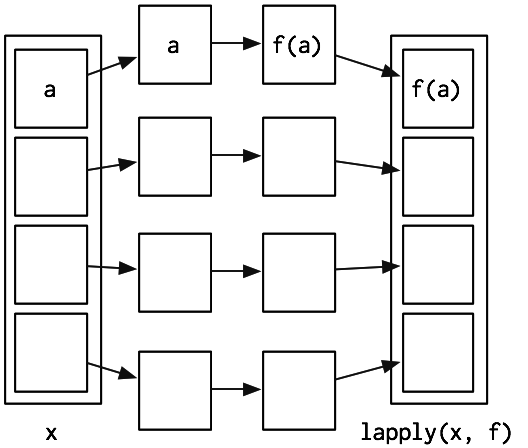
\includegraphics[scale=0.8]{figures/lapply}	\\
		\end{center}
	\end{figure}
\end{frame}

\begin{frame}
	\frametitle{parallel package}
	Two approaches:
	\begin{center}
		\begin{enumerate}
			\item mclapply()
			\item parLapply()
		\end{enumerate}
	\end{center}
\end{frame}

\begin{frame}
	\frametitle{mclapply()}
	\begin{center}
		\textbf{Pros} \\
		Simple to use \\
		Low overhead (startup) \\~\\
		
		\textbf{Cons} \\
		Does not work on Windows \\
		Only multi core \\
	\end{center}
\end{frame}

\begin{frame}
	\frametitle{parLapply(type=''psock'')}
	\begin{center}
		\textbf{Pros} \\
		Works everywhere \\
		Good for testing/developing \\~\\
		
		\textbf{Cons} \\
		Slow on multiple nodes
	\end{center}
\end{frame}

\begin{frame}
	\frametitle{parLapply(type=''mpi'')}
	\begin{center}
		\textbf{Pros} \\
		Good for multiple computers
		Good for production \\~\\
		
		\textbf{Cons} \\
		Can be used interactively
		Needs Rmpi package
	\end{center}
\end{frame}

\begin{frame}
	\frametitle{Example}
	\begin{center}
		\href{https://github.com/MansMeg/AdvRCourse/blob/master/Code/parallel_example.R}{example}
	\end{center}
\end{frame}

%------------------------------------------------
\section{Rcpp}
%------------------------------------------------

\begin{frame}
	\frametitle{Rcpp}
	\begin{center}
		Using C++ code in R \\~\\
		Need C++ compiler (look \href{http://adv-r.had.co.nz/Rcpp.html}{here}) 
		\\~\\
		Often called interfacing \\~\\
		Similar can be done with Java and Fortran \\~\\
		Extremely fast! \\~\\
		But just handle bottlenecks! \\~\\
	\end{center}
\end{frame}

\defverbatim[colored]\lstRFac{
\begin{lstlisting}[language=R,basicstyle=\ttfamily,keywordstyle=\color{black}]
	fr <- function(n) {
	  if (n < 2) return(n)
	  f(n-1) + f(n-2)
	}
	
	
	system.time(fr(30))
	user  system elapsed 
	2.246   0.171   2.451 
\end{lstlisting}
}

\begin{frame}
	\frametitle{Fibonacci}
	\begin{center}
\[
f(n)= 
\begin{cases}
	n, & \text{if } n \textless 2 \\
	F(n - 1) + F(n - 2), & \text{otherwise}
\end{cases}
\]
\end{center}
\end{frame}

\begin{frame}
	\frametitle{Fibonacci R}
	\lstRFac
\end{frame}

\defverbatim[colored]\lstCPPFac{
	\begin{lstlisting}[language=R,basicstyle=\ttfamily,keywordstyle=\color{black},showstringspaces=false]
	library(Rcpp)
	
	cppFunction(code = '
	  int fcpp(int n) { 
	    if (n < 2) return(n); 
	    return(fcpp(n-1) + fcpp(n-2)); 
	  }
	')
	
	system.time(fcpp(30))
	user      system     elapsed 
	0.007000000 0.000000000 0.006999999 
	\end{lstlisting}
}

\begin{frame}
	\frametitle{Fibonacci C++}
	\lstCPPFac
\end{frame}

%------------------------------------------------
\section{Memoization}
%------------------------------------------------

\begin{frame}
	\frametitle{Memoization}
	\begin{center}
		A simple optimization technique \\
		Example of a general technique in optimization of trading memory for 
		computation\\~\\
		Memoization stores (caches) results of function calls \\~\\
		If called again, returns old value \\~\\
		Depends on functional programming \\~\\
	\end{center}
\end{frame}

\defverbatim[colored]\lstMem{
	\begin{lstlisting}[language=R,basicstyle=\ttfamily,keywordstyle=\color{black},showstringspaces=false]
> library(memoise)
> a <- function(x) runif(1)
> replicate(3, a())
[1] 0.6709919 0.3490709 0.4772027
> b <- memoise(a)
> replicate(3, b())
[1] 0.1867441 0.1867441 0.1867441
	\end{lstlisting}
}

\begin{frame}
	\frametitle{Memoise in R}
	\lstMem
\end{frame}

\defverbatim[colored]\lstMemRun{
	\begin{lstlisting}[language=R,basicstyle=\ttfamily\small,keywordstyle=\color{black},showstringspaces=false]
> c <- memoise(function(x) {Sys.sleep(1); runif(1)})
> system.time(print(c()))
[1] 0.7816399
user  system elapsed 
0.003   0.004   1.001 
> system.time(print(c()))
[1] 0.7816399
user  system elapsed 
0.001   0.000   0.000 
> forget(c)
[1] TRUE
> system.time(print(c()))
[1] 0.9234995
user  system elapsed 
0.003   0.004   1.001 
\end{lstlisting}
}

\begin{frame}
	\frametitle{Memoise in R}
	\lstMemRun
\end{frame}

%------------------- THE END ---------------------------------------------------

\begin{frame}
\Huge{\centerline{The End... for today.}}
\Huge{\centerline{Questions?}}
\Huge{\centerline{See you next time!}}
\end{frame}

%-------------------------------------------------------------------------------

\end{document} 